\chapter{Dados do sistema de 24 nós}
\label{anex:24barras}
O sistema de distribuição de 24 nós utilizado neste trabalho é o mesmo utilizado em \citeonline{MunozDelgado2015}, porém, não é considerado os geradores distribuídos eólicos. Este opera em 20kV e possui 20 nós de carga e 4 nós de subestações (sendo dois deles já existentes), 29 ramos candidatos à instalação, 2 ramos existentes fixos e 2 ramos existentes que podem ser substituíveis, totalizando 33 ramos. A figura \ref{fig:24bus} apresenta o diagrama unifilar do sistema de distribuição, bem como os nós que podem receber geradores distribuídos operados pela empresa de distribuição.
\begin{figure}[ht]
 	\centering
    \caption{Diagrama unifilar do sistema de 24 nós.}
    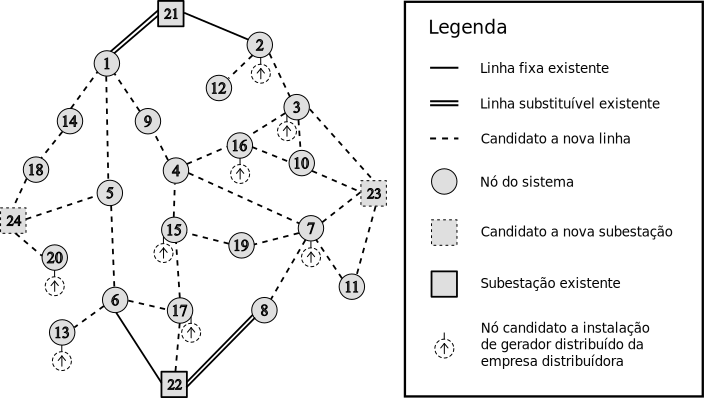
\includegraphics[width=0.8\textwidth]{Anexos/24-bus-system.pdf}\\
    Fonte: Adaptado de \citeonline{MunozDelgado2015}
    \label{fig:24bus}
\end{figure}


Este sistema de distribuição passa por 3 estágios e 3 níveis de carregamento. A tabela \ref{tab:param_carga} apresenta a demanda máxima de cada nó de carga em cada estágio. Note que metade dos barramentos possuem carga já no final do primeiro estágio.
\begin{table}[ht]
\centering
\caption{Demanda máxima do sistema (MVA).}
\label{tab:param_carga}
\begin{tabular}{@{}cccccccc@{}}
\toprule
\multirow{2}{*}{Nó} & \multicolumn{3}{c}{Estágio} & \multirow{2}{*}{Nó} & \multicolumn{3}{c}{Estágio} \\ \cmidrule(lr){2-4} \cmidrule(l){6-8} 
   & 1    & 2    & 3    &    & 1 & 2    & 3    \\ \midrule
1  & 4,05 & 3,45 & 5,42 & 11 & 0 & 1,91 & 2,8  \\
2  & 0,78 & 0,77 & 1,21 & 12 & 0 & 0,93 & 1,29 \\
3  & 2,58 & 3,38 & 3,98 & 13 & 0 & 1,15 & 1,87 \\
4  & 0,32 & 0,41 & 2,43 & 14 & 0 & 3,05 & 3,16 \\
5  & 0,28 & 0,37 & 0,47 & 15 & 0 & 1,62 & 1,62 \\
6  & 1,17 & 0,92 & 1,81 & 16 & 0 & 2,16 & 1,22 \\
7  & 4,04 & 3,7  & 4,36 & 17 & 0 & 0    & 2,4  \\
8  & 0,72 & 0,6  & 0,94 & 18 & 0 & 0    & 2,1  \\
9  & 1,14 & 1,12 & 1,77 & 19 & 0 & 0    & 1,81 \\
10 & 1,56 & 2,04 & 2,4  & 20 & 0 & 0    & 3,79 \\ \bottomrule
\end{tabular}
\\Fonte: Adaptado de \citeonline{MunozDelgado2015}
\end{table}

Já na tabela \ref{tab:param_ramos} são apresentados os comprimentos de cada ramo do sistema, incluindo os ramos existentes.
\begin{table}[ht]
\centering
\caption{Dados dos comprimentos dos ramos (km).}
\label{tab:param_ramos}
\begin{tabular}{@{}ccccccccc@{}}
\toprule
Nó & Nó & Comprimento & Nó & Nó & Comprimento & Nó & Nó & Comprimento \\ \midrule
1  & 5  & 2,22        & 4  & 9  & 1,2         & 7  & 23 & 0,9         \\
1  & 9  & 1,2         & 4  & 15 & 1,6         & 8  & 22 & 1,9         \\
1  & 14 & 1,2         & 4  & 16 & 1,3         & 10 & 16 & 1,6         \\
1  & 21 & 2,2         & 5  & 6  & 2,4         & 10 & 23 & 1,3         \\
2  & 3  & 2           & 5  & 24 & 0,7         & 11 & 23 & 1,6         \\
2  & 12 & 1,1         & 6  & 13 & 1,2         & 14 & 18 & 1           \\
2  & 21 & 1,7         & 6  & 17 & 2,2         & 15 & 17 & 1,2         \\
3  & 10 & 1,1         & 6  & 22 & 2,7         & 15 & 19 & 0,8         \\
3  & 16 & 1,2         & 7  & 8  & 2           & 17 & 22 & 1,5         \\
3  & 23 & 1,2         & 7  & 11 & 1,1         & 18 & 24 & 1,5         \\
4  & 7  & 2,6         & 7  & 19 & 1,2         & 20 & 24 & 0,9         \\ \bottomrule
\end{tabular}
\\Fonte: Adaptado de \citeonline{MunozDelgado2015}
\end{table}

As tabelas \ref{tab:param_trafo}, \ref{tab:param_dg} e \ref{tab:param_linha} apresentam respectivamente os dados dos transformadores, geradores distribuídos e linhas que podem ser instalados neste sistema de distribuição.
\begin{table}[ht]
\centering
\caption{Parâmetros dos candidatos a novos transformadores}
\label{tab:param_trafo}
\begin{tabular}{@{}cccccccc@{}}
\toprule
\multicolumn{4}{c}{Alternativa 1} & \multicolumn{4}{c}{Alternativa 2} \\ \midrule
$\overline{G}^{NT}_1$ & $Z^{NT}_1$ & $C^{M,NT}_1$ & $C^{I,NT}_1$ & $\overline{G}^{NT}_2$ & $Z^{NT}_2$ & $C^{M,NT}_2$ & $C^{I,NT}_2$ \\
(MVA)  & ($\Omega$)  & (USD) & (USD)   & (MVA)  & ($\Omega$)  & (USD) & (USD)   \\ \midrule
12     & 0,16     & 2000 & 750000 & 15     & 0,13     & 3000 & 950000 \\ \bottomrule
\end{tabular}
\\Fonte: Adaptado de \citeonline{MunozDelgado2015}
\end{table}
\begin{table}[ht]
\centering
\caption{Parâmetros dos candidatos a novos geradores distribuídos}
\label{tab:param_dg}
\begin{tabular}{@{}cccccccc@{}}
\toprule
\multicolumn{4}{c}{Alternativa 1}     & \multicolumn{4}{c}{Alternativa 2}     \\ \midrule
$\overline{G}^{DG}_1$ & $C^{I,DG}_1$ & $C^{M,DG}_1$ & $C^{E,DG}_1$ & $\overline{G}^{DG}_2$ & $C^{I,DG}_2$ & $C^{M,DG}_2$ & $C^{E,DG}_2$ \\
(MVA) & ($\frac{\text{USD}}{\text{MWh}}$) & (USD) & ($\frac{\text{USD}}{\text{MWh}}$) & (MVA) & ($\frac{\text{USD}}{\text{MWh}}$)& (USD) & ($\frac{\text{USD}}{\text{MWh}}$) \\ \midrule
1     & 500000    & 22500 & 47        & 2     & 490000    & 44100 & 45        \\ \bottomrule
\end{tabular}
\end{table}
\begin{table}[ht]
\centering
\caption{Parâmetros dos candidatos a linhas}
\label{tab:param_linha}
\begin{tabular}{@{}ccccccc@{}}
\toprule
\multirow{2}{*}{Tipo} & \multicolumn{3}{c}{Alternativa 1}              & \multicolumn{3}{c}{Alternativa 2}              \\ \cmidrule(l){2-7} 
                      & $\overline{F}^{l}_1$ & $Z^{l}_1$ & $C^{I,l}_1$ & $\overline{F}^{l}_2$ & $Z^{l}_2$ & $C^{I,l}_2$ \\ \midrule
$l$ & (MVA) & ($\frac{\Omega}{\text{km}}$) & ($\frac{\text{USD}}{\text{km}}$) & (MVA) & ($\frac{\Omega}{\text{km}}$) & ($\frac{\text{USD}}{\text{km}}$) \\ \midrule
$NRB$                 & 6,28                 & 0,557     & 19140       & 9                    & 0,478     & 29870       \\ \midrule
$NAB$                 & 3,94                 & 0,732     & 15020       & 6,28                 & 0,557     & 25030       \\ \bottomrule
\end{tabular}
\end{table}

\newpage
A tabela \ref{tab:param_carrega} apresenta os dados que se referem ao nível de carregamento do sistema, como o fator de carregamento, duração estimada do nível de carga e custo de compra de energia no nível de carga.
\begin{table}[ht]
\centering
\caption{Parâmetros por nível de carregamento.}
\label{tab:param_carrega}
\begin{tabular}{@{}lccccc@{}}
\toprule
                              &            & \multicolumn{3}{c}{Nível de carregamento} &         \\ \cmidrule(l){2-6} 
Descrição                         & Símbolo    & 1             & 2             & 3             & Unidade \\ \midrule
Fator de carregamento         & $\mu_b$    & 70            & 83            & 100           & \%      \\
Duração estimada              & $\Delta_b$ & 2000          & 5760          & 1000          & h/ano   \\
Custo de energia da subestção & $C^{SS}_b$ & 57,7          & 70            & 85,3          & USD/MWh \\ \bottomrule
\end{tabular}
\\Fonte: Adaptado de \citeonline{MunozDelgado2015}
\end{table}

Por fim, a tabela \ref{tab:param} apresenta outros dados utilizados neste sistema, incluindo os dados financeiros, ativos já instalados, vida útil, etc.
\begin{table}[ht]
\centering
\caption{Parâmetros gerais utilizados}
\label{tab:param}
\begin{tabular}{@{}llccc@{}}
\toprule
 &
  Descrição &
  Símbolo &
  Valor &
  Unidade \\ \midrule
 &
  Taxa de juros &
  $i$ &
  7,1 &
  \% \\
 &
   &
   &
  \multicolumn{1}{l}{} &
  \multicolumn{1}{l}{} \\
 &
  Limite de orçamento &
  $IB_t; \; \forall t \in T$ &
  \multicolumn{1}{l}{6 milhões} &
  USD \\
 &
   &
   &
  \multicolumn{1}{l}{} &
  \multicolumn{1}{l}{} \\
 &
  \begin{tabular}[c]{@{}l@{}}Limite de penetração\\ de geradores\\ distribuídos\end{tabular} &
  $\xi$ &
  25 &
  \% \\
 &
   &
   &
  \multicolumn{1}{l}{} &
  \multicolumn{1}{l}{} \\
 &
  Fator de potência &
  $pf$ &
  0,9 &
  - \\
 &
   &
   &
  \multicolumn{1}{l}{} &
  \multicolumn{1}{l}{} \\
 &
  Tensão base &
  - &
  20 &
  kV \\
 &
   &
   &
  \multicolumn{1}{l}{} &
  \multicolumn{1}{l}{} \\
 &
  \begin{tabular}[c]{@{}l@{}}Limite de tensão \\ superior\end{tabular} &
  $\overline{V}$ &
  1,05 &
  p.u. \\
 &
   &
   &
  \multicolumn{1}{l}{} &
  \multicolumn{1}{l}{} \\
 &
  \begin{tabular}[c]{@{}l@{}}Limite de tensão \\ inferior\end{tabular} &
  $\underline{V}$ &
  0,95 &
  p.u. \\ \midrule
\multirow{7}{*}{\begin{tabular}[c]{@{}l@{}}Dados dos \\ ativos já \\ instalados\end{tabular}} &
  \begin{tabular}[c]{@{}l@{}}Impedância dos \\ transformadores\end{tabular} &
  $Z^{ET}_k; \; \forall k \in K^{ET}$ &
  0,25 &
  $\Omega$ \\
 &
   &
   &
  \multicolumn{1}{l}{} &
  \multicolumn{1}{l}{} \\
 &
  \begin{tabular}[c]{@{}l@{}}Potência nominal \\ dos transformadores\end{tabular} &
  $\overline{G}^{ET}_k; \; \forall k \in K^{ET}$ &
  7,5 &
  MVA \\
 &
   &
   &
  \multicolumn{1}{l}{} &
  \multicolumn{1}{l}{} \\
 &
  \begin{tabular}[c]{@{}l@{}}Ampacidade \\ das linhas\end{tabular} &
  \begin{tabular}[c]{@{}c@{}}$\overline{F}^{l}_k;$\\ $\forall l \in \{EFB,ERB\}, \forall k \in K^{l}$\end{tabular} &
  3,94 &
  MVA \\
 &
   &
   &
  \multicolumn{1}{l}{} &
  \multicolumn{1}{l}{} \\
 &
  \begin{tabular}[c]{@{}l@{}}Impedância \\ das linhas\end{tabular} &
  \begin{tabular}[c]{@{}c@{}}$\overline{Z}^{l}_k; $\\ $\forall l \in \{EFB,ERB\}, \forall k \in K^{l}$\end{tabular} &
  0,732 &
  $\Omega$/km \\ \midrule
\multirow{7}{*}{Vida útil} &
  Subestação &
  $\eta^{SS}$ &
  $\infty^+$ &
  anos \\
 &
   &
   &
  \multicolumn{1}{l}{} &
  \multicolumn{1}{l}{} \\
 &
  Transformador &
  $\eta^{NT}$ &
  15 &
  anos \\
 &
   &
   &
  \multicolumn{1}{l}{} &
  \multicolumn{1}{l}{} \\
 &
  Linhas &
  $\eta^{l}; \;\forall l \in \{NAB, NRB\}$ &
  25 &
  anos \\
 &
   &
   &
  \multicolumn{1}{l}{} &
  \multicolumn{1}{l}{} \\
 &
  Geradores distribuídos &
  $\eta^{DG}$ &
  20 &
  anos \\ \midrule
\multirow{5}{*}{Quantidades} &
  Estágios &
  $n_T$ &
  3 &
  - \\
 &
   &
   &
  \multicolumn{1}{l}{} &
  \multicolumn{1}{l}{} \\
 &
  \begin{tabular}[c]{@{}l@{}}Nós candidatos a \\ receber geradores \\ distribuídos\end{tabular} &
  $n_{DG}$ &
  8 &
  - \\
 &
   &
   &
  \multicolumn{1}{l}{} &
  \multicolumn{1}{l}{} \\
 &
  Partes da linearização &
  $n_\nu$ &
  3 &
  - \\ \bottomrule
\end{tabular}
Fonte: Adaptado de \citeonline{MunozDelgado2015}
\end{table}
